\subsection{Steps to Implement a Fair-by-Design Workflow}
\label{subsection:steps}

\begin{enumerate}

    \item \emph{Objective Definition:} Clearly articulate the objectives of the system or process being designed, emphasizing the importance of fairness.

    \item \emph{Stakeholder Identification:} Identify and involve key stakeholders, ensuring a diverse representation that reflects the potential impacts of the system.

    \item \emph{Data Collection:} Determine the types of data needed for the application, establish ethical data collection protocols.

    \item \emph{Data pre-processing:} Prepare the data for the fairness algorithm, through data cleaning and featyre engineering
    
    \item \emph{Algorithmic Design and Definitions:} Define and implement fairness-enhancing algorithms across pre-processing, in-processing, and post-processing stages. Provide detailed definitions and explanations for each algorithm.

    \item \emph{Model training and evaluation:} Define the training step, performs the training tuning certain parameters and provides an evaluation of the performances of the models based on accuracy and fairness metrics.

    \item \emph{Model deployment:} Define the change of the environment of the model from a development environment to real world application environment.

\end{enumerate}

It's important to clarify the workflow concept with a graph illustrating the presented workflow:

\begin{figure}[h]
    \centering
    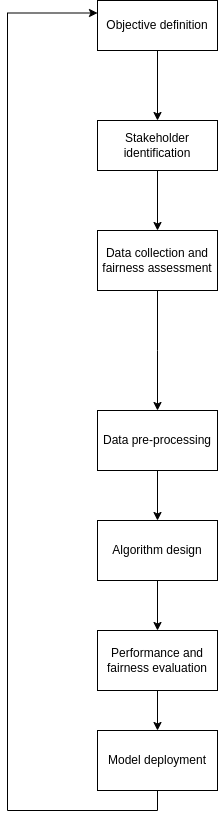
\includegraphics[width=.5\textwidth,height=1\textwidth]{final.png}
    \caption{Fair-by-Design Workflow}
\end{figure}

In the subsequent sections, each of these steps will be comprehensively explored to provide a detailed understanding of the fair-by-design workflow and its ethical underpinnings.
